\documentclass[letterpaper,12pt]{article}
\usepackage[bottom=2.5cm, top=2.5cm, right=2cm, left=3cm]{geometry}
\usepackage[spanish, es-tabla]{babel}
\usepackage{graphicx} 
\usepackage{hyperref}
\usepackage{booktabs}
\usepackage{natbib}
\usepackage{float}
\usepackage{listings}
\usepackage{xcolor}
\usepackage{parskip} 
\usepackage{fancyhdr} % Paquete para personalizar encabezados y pies de página
\usepackage{microtype}  % Mejora la justificación del texto

\hypersetup{
    colorlinks=true,
    linkcolor=black,
    citecolor=black,
    urlcolor=blue
}

% Configuración del encabezado
\pagestyle{fancy}
\fancyhf{} % Limpia los encabezados y pies de página actuales
\fancyhead[R]{\thepage} % Coloca el número de página en la parte superior derecha
\renewcommand{\headrulewidth}{0pt} % Elimina la línea horizontal en la parte superior de la página

\begin{document}

\begin{titlepage}
    \begin{center}
      \vspace*{1cm}

    \textbf{\Large DISTRIBUCIÓN DE VIAJES EN SAN CARLOS DE APOQUINDO}
    
    \vspace{1cm}
    
    \textbf{Bernardo Caprile Canala-Echevarría}\\
    Facultad de Ingeniería y Ciencias Aplicadas, Universidad de los Andes, Santiago de Chile\\
    e-mail: \href{mailto:bcaprile@miuandes.cl}{bcaprile@miuandes.cl}
    
    \vspace{2cm}
    
    \textbf{RESUMEN}
    
    \vspace{0.5cm}  
    \end{center}
    
    \textit{Palabras clave:}
\end{titlepage}

\newpage

\section{Introducción}

El flujo de vehículos en hora punta de la mañana en San Carlos de Apoquindo es un problema significativo, ya que esta zona, además de ser un barrio residencial, se caracteriza por tener una alta concentración de colegios y universidades. Por lo tanto, el tráfico matutino afecta tanto a los residentes como a los estudiantes que ingresan a esta área. Para poder tomar decisiones respecto al flujo vehicular, no solo en San Carlos de Apoquindo, sino en todo Santiago, se realiza periódicamente la encuesta origen-destino, la cual permite conocer la cantidad de viajes que se realizan en la ciudad y su distribución.

Con esta información, se pueden generar modelos y tomar decisiones, las cuales optimicen las rutas de las personas, disminuyendo el tráfico y el tiempo de viaje. Por esta razón, es importante contar con una matriz origen-destino actualizada y precisa, la cual permita realizar análisis y proyecciones de la distribución de viajes en la ciudad. A continuación, se presenta la figura \ref{fig:mapa}, la cual muestra la zonificación de una parte de Las Condes enfocada en San Carlos de Apoquindo. 

\begin{figure}[h!]
    \centering
    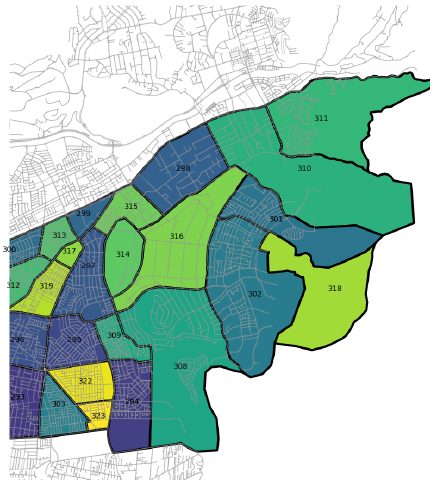
\includegraphics[width=0.5\textwidth]{fotos/mapa.png}
    \caption{Mapa de San Carlos de Apoquindo.}
    \label{fig:mapa}
\end{figure}

Para esta tarea, se generarán 3 matrices origen-destino en base a esta zonificación mediante un código Python: una utilizando el método Furness o biproporcional, con datos de los vectores origen-destino de 2024, otra a partir de una matriz de costos, como la distancia promedio de viaje, y el modelo gravitacional. Posteriormente, se calibrará la matriz con el modelo gravitacional y se compararán los resultados obtenidos con un error cuadrático medio respecto a la matriz original. Finalmente, a la matriz calibrada se le aplicará el método de Furness para obtener una matriz de viajes.













\end{document}
